\documentclass[unicode,11pt,a4paper,oneside,numbers=endperiod,openany]{scrartcl}
\usepackage{listings}
\usepackage{amsmath}

\renewcommand{\thesubsection}{\arabic{subsection}}

\usepackage{ifthen}
\usepackage[utf8]{inputenc}
\usepackage{graphics}
\usepackage{graphicx}
\usepackage{hyperref}

\pagestyle{plain}
\voffset -5mm
\oddsidemargin  0mm
\evensidemargin -11mm
\marginparwidth 2cm
\marginparsep 0pt
\topmargin 0mm
\headheight 0pt
\headsep 0pt
\topskip 0pt        
\textheight 255mm
\textwidth 165mm

\newcommand{\duedate} {}
\newcommand{\setduedate}[1]{%
\renewcommand\duedate {\textbf{Due date:}~ #1}}
\newcommand\isassignment {false}
\newcommand{\setassignment}{\renewcommand\isassignment {true}}
\newcommand{\ifassignment}[1]{\ifthenelse{\boolean{\isassignment}}{#1}{}}
\newcommand{\ifnotassignment}[1]{\ifthenelse{\boolean{\isassignment}}{}{#1}}

\newcommand{\assignmentpolicy}{
\begin{table}[h]
\begin{center}
\scalebox{0.8} {%
\begin{tabular}{|p{0.02cm}p{16cm}|}
\hline
&\\
\multicolumn{2}{|c|}{\Large\textbf{Numerical Computing 2023 ---  Submission Instructions}}\\
\multicolumn{2}{|c|}{\large\textbf{(Please, notice that following instructions are mandatory: }}\\
\multicolumn{2}{|c|}{\large\textbf{submissions that don't comply with, won't be considered)}}\\
&\\
\textbullet & Assignments must be submitted to \href{https://www.icorsi.ch/course/view.php?id=14666}{iCorsi} (i.e. in electronic format).\\
\textbullet & Provide both executable package and sources (e.g. C/C++ files, MATLAB). 
If you are using libraries, please add them in the file. Sources must be organized in directories called:\\
\multicolumn{2}{|c|}{\textit{Project\_number\_lastname\_firstname}}\\
& and  the  file must be called:\\
\multicolumn{2}{|c|}{\textit{project\_number\_lastname\_firstname.zip}}\\
\multicolumn{2}{|c|}{\textit{project\_number\_lastname\_firstname.pdf}}\\
\textbullet &  The TAs will grade your project by reviewing your project write-up, and looking at the implementation you attempted, and benchmarking your code's performance.\\

\textbullet & You are allowed to discuss all questions with anyone you like; however: (i) your submission must list anyone you discussed problems with and (ii) you must write up your submission independently.\\
\hline
\end{tabular}
}
\end{center}
\end{table}
}
\newcommand{\punkte}[1]{\hspace{1ex}\emph{\mdseries\hfill(#1~\ifcase#1{Points}\or{Points}\else{Points}\fi)}}


\newcommand\serieheader[6]{
\thispagestyle{empty}%
\begin{flushleft}

\includegraphics[width=0.45\textwidth]{CI_logo}
\end{flushleft}
  \noindent%
  {\large\ignorespaces{\textbf{#1}}\hspace{\fill}\ignorespaces{ \textbf{#2}}}\\ \\%
  {\large\ignorespaces #3 \hspace{\fill}\ignorespaces #4}\\
  \noindent%
  \bigskip
  \hrule\par\bigskip\noindent%
  \bigskip {\ignorespaces {\Large{\textbf{#5}}}
  \hspace{\fill}\ignorespaces \large \ifthenelse{\boolean{\isassignment}}{\duedate}{#6}}
  \hrule\par\bigskip\noindent%  \linebreak
 }

\makeatletter
\def\enumerateMod{\ifnum \@enumdepth >3 \@toodeep\else
      \advance\@enumdepth \@ne
      \edef\@enumctr{enum\romannumeral\the\@enumdepth}\list
      {\csname label\@enumctr\endcsname}{\usecounter
        {\@enumctr}%%%? the following differs from "enumerate"
	\topsep0pt%
	\partopsep0pt%
	\itemsep0pt%
	\def\makelabel##1{\hss\llap{##1}}}\fi}
\let\endenumerateMod =\endlist
\makeatother




\usepackage{textcomp}





\begin{document}


\setassignment
\setduedate{Wednesday, 6 December 2023, 11:59 PM}

\serieheader{Numerical Computing}{2023}{\textbf{Student:} FULL NAME}{\textbf{Discussed with:} FULL NAME}{Solution for Project 4}{}
\newline

\assignmentpolicy


\newpage

\section{General Questions [10 points]}

\begin{enumerate}
 \item What is the size of the matrix A? \\
 
 The size of matrix A stored in 'blurred\_data' folder is \textbf{62500 X 62500}. The result is obtained as following: \\
 
 \begin{lstlisting}[language=Matlab]
% Load the matrix struct
load('blured_data/A.m'); 

% Get the size of matrix A loaded
sizeA = size(A);

... print the matrix size...
 \end{lstlisting}
 
 It can also be calculated manually as we know the value of ${n = 250}$, and as A is ${n^2}$ X ${n^2}$ matrix A is going to be ${250^2}$ X ${250^2}$ which is \textbf{62500 X 62500}.
 
 \vspace{20px}
 
 \item How many diagonal bands does A have? \\
 
 We have a kernel matrix with the size of 7 X 7. As (${d \leq n}$), and ${n=7}$, the ${d}$ can be set as 7. As the matrix is ${d^2}$-matrix, the number of diagonal bands in A is equal to ${d^2}$ which is 49.
 
 \vspace{20px}
 
 \item What is the length of the vectorized blurred image in b? \\
 
 Matrix A operates on a "row-vectorized" image matrix. In this case, the length of the vectorized blurred image in b would be equivalent to ${len(b)=n\times n}$. As ${n = 250}$, length of ${b}$ would be ${250 \times 250 = 625,000}$.
\vspace{20px}
\end{enumerate}


\section{Properties of A [10 points]}

\begin{enumerate}
 \item If A is not symmetric, how would this affect ${\tilde{A}}$? \\
 
  \begin{equation}
  A^TAx = A^Tb
 \end{equation}
 \begin{equation}
  \tilde{A}x = \tilde{b}
 \end{equation}

The operation in equation 1 needs to be performed in case the coefficient matrix ${A}$ is not positive-definite like the case we have, as the Conjugate Gradient method requires the coefficient matrix to be positive-definite. However, during this operation, conditional number ${\kappa(A)}$ gets effected because ${\kappa (\tilde{A}) = {\kappa(A)}^2}$. The counterpart of ${A}$ is symmetric as it is a square matrix formed from product of ${B^TB}$, hence, matrix ${A}$ also has to be symmetric. \\

\newpage
\item Explain why solving ${Ax = b}$ for x is equivalent to minimizing ${\frac{1}{2}x^TAx - b^Tx}$ over x, assuming that A is symmetric positive-definite. \\

The minimum of the given equation can be easily computed by computing the derivative of the equation: \\

\begin{equation*}
f'(x) = \frac{d}{dx}(\frac{1}{2}x^TAx - b^Tx) \\
\end{equation*}
\begin{equation*}
\hspace*{20px}= \frac{1}{2}A^Tx + \frac{1}{2}Ax - b
\end{equation*}

Because ${A}$ is symmetric, we can assume ${A = A^T}$, and we can replace ${A^T}$ with ${A}$.

\begin{equation*}
\hspace*{20px}= \frac{1}{2}Ax + \frac{1}{2}Ax - b
\end{equation*}

And it can be simplified to ${Ax - b}$. A function's minimum lies where the ${f'(x) = 0}$, hence the minimum of the given function can be found when:

\begin{equation*}
 Ax - b = 0
\end{equation*}

Which is equivalent to :
\begin{equation*}
 Ax = b
\end{equation*}
\end{enumerate}


\section{Conjugate Gradient [30 points]}

\begin{enumerate}
 \item Write a function for the conjugate gradient solver ${[x,rvec]=myCG(A,b,x0,max\_itr,tol)}$, where x
and rvec are, respectively, the solution value and a vector containing the residual at every iteration. \\

Conjugate Gradient solver is an iterative method of solving a large linear system to get a approximated solution. Our implementation takes ${A}$ the system matrix, ${b}$ the row-vectorized vector, ${x0}$ the initial guess, ${max\_itr}$ the maximum number of iterations, ${tol}$ the tolerance for convergence, and output the ${x}$ which is the solution to equation 2 with the residual norms of each iteration as ${rvec}$. The implementation is as following:

\begin{lstlisting}[language=Matlab]
 function [x, rvec] = myCG(A, b, x0, max_itr, tol)
    rvec = [];
    x = x0;
    r = b - A * x;
    d = r;
    p_old = dot(r, r);
    for i = 1:max_itr
        s = A * d;
        alpha = p_old / dot(d, s);
        x = x + alpha * d;
        r = r - alpha * s;
        p_new = dot(r, r);
        beta = p_new / p_old;
        d = r + beta * d;
        p_old = p_new;
        rvec = [rvec, p_new];
        if sqrt(p_new) <= tol
            disp('Converged');
            break;
        end
    end
end
\end{lstlisting}

\item In order to validate your implementation, solve the system defined by ${A\_test.mat}$ and ${b\_test.mat}$. Plot
the convergence (residual vs iteration).
\vspace{20px}

Implementation is as the following:

\begin{lstlisting}[language=Matlab]
load('test_data/A_test.mat', 'A_test');
load('test_data/b_test.mat', 'b_test');

m = sqrt(length(b_test));
n = m;

guess=zeros(size(A_test, 1), 1);
max_itr = 200;
tol = 1e-4;

[x, rvec] = myCG(A_test, b_test, guess, max_itr, tol);
...plot the graph...
\end{lstlisting}
\vspace{20px}

The resulting graph is as the following:

 \begin{figure}[h!]
    \begin{minipage}[c]{1\linewidth}
        \centering
        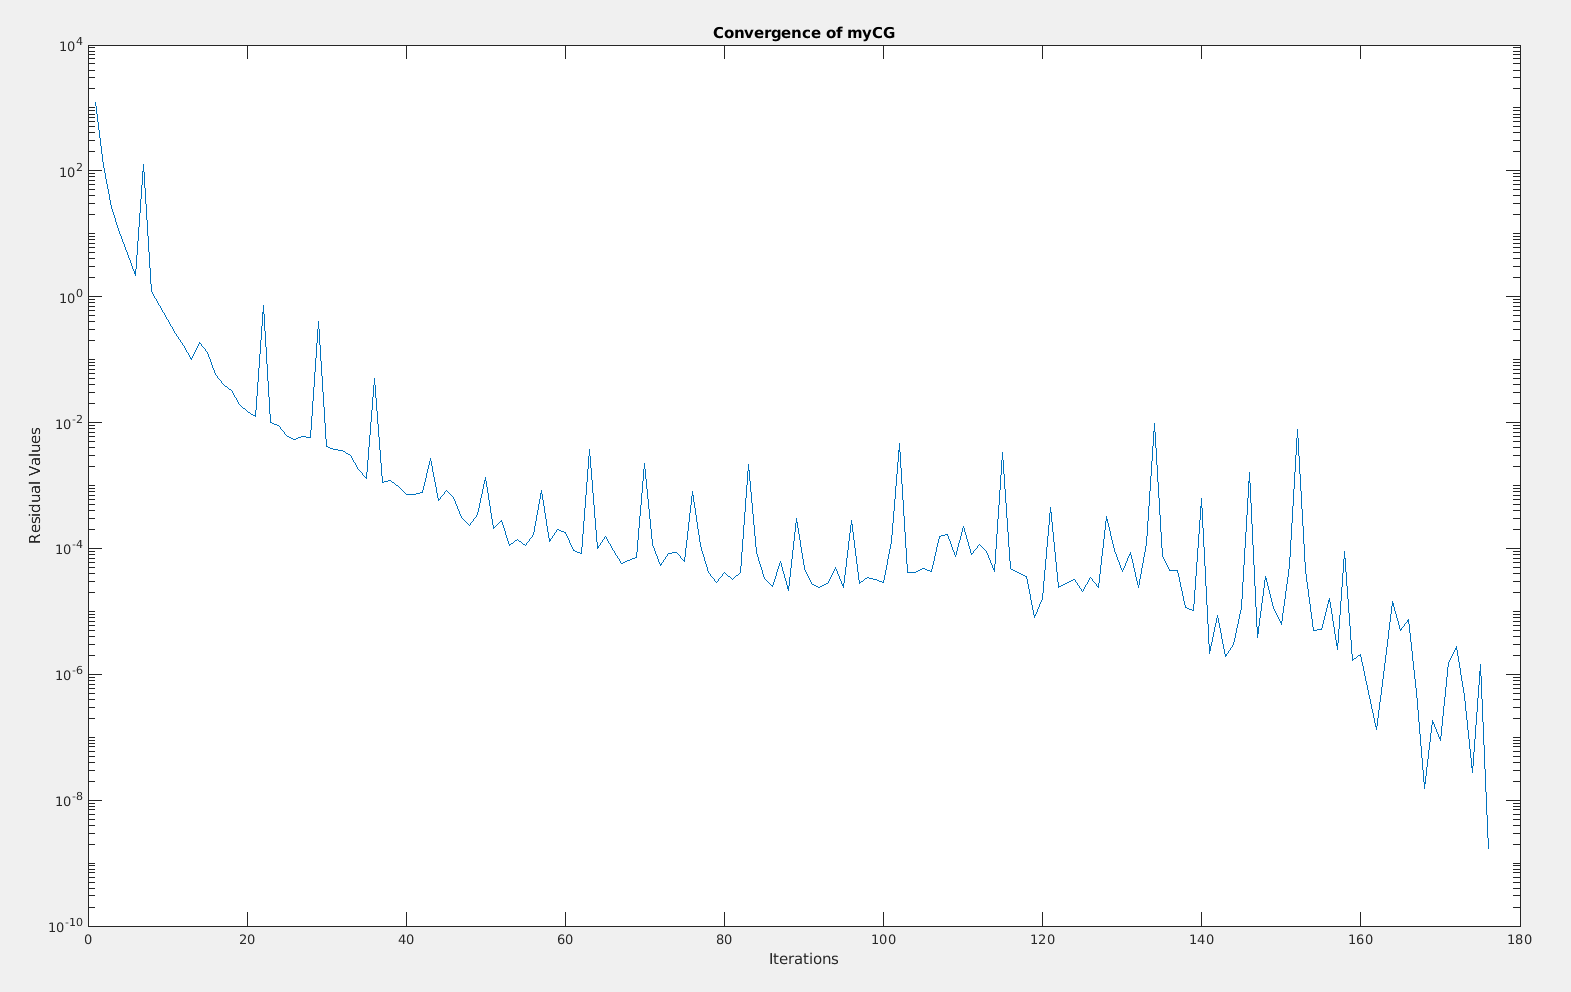
\includegraphics[width=0.9\linewidth]{./figures/ex3b.png}
    \end{minipage}
  \caption{Plotted residual values against iteration using myCG function}
\end{figure}

The implementation of Conjugate Gradient (myCG) seems to find the convergence of the test data very quickly under 200 iterations. 

\newpage

\item Plot the eigenvalues of ${A\_test.mat}$ and comment on the condition number and convergence rate. \\
 \begin{figure}[h!]
    \begin{minipage}[c]{1\linewidth}
        \centering
        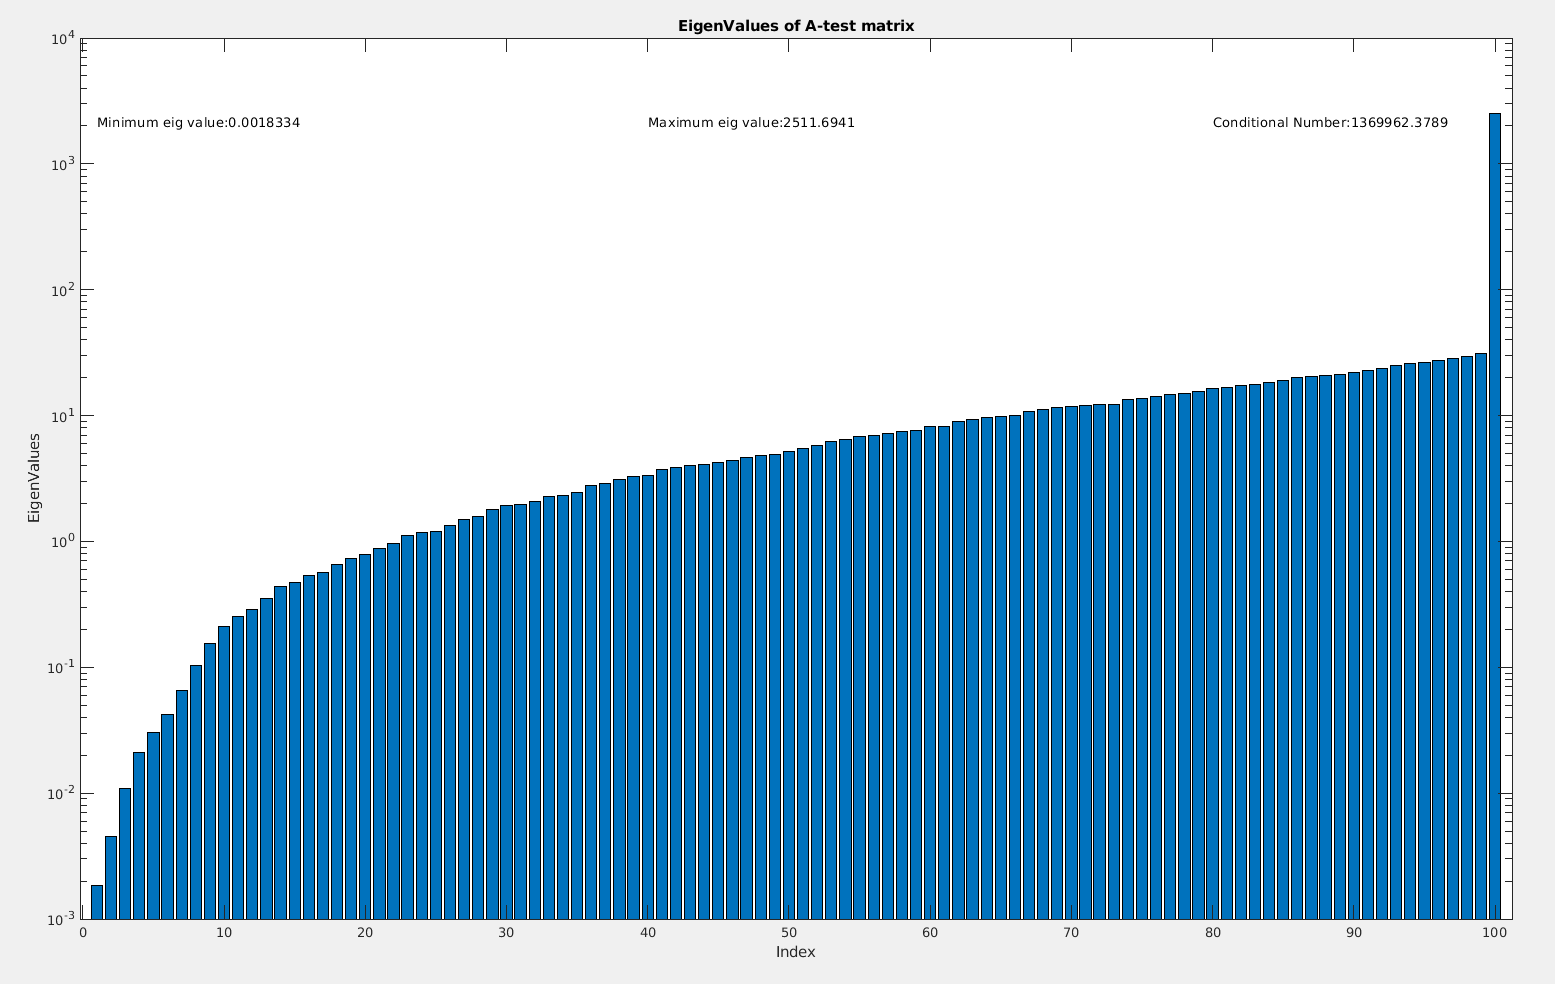
\includegraphics[width=0.9\linewidth]{./figures/ex3c.png}
    \end{minipage}
  \caption{Eigen value distribution in matrix A\_test.mat (Eigen values are logged for better visualization)}
\end{figure}

Implementation can be seen in ${ex3c.m}$ file in the data folder.

As it can be seen from the plotting, there is a significant difference between the smallest and the largest absolute eigenvalues. As a result, it results in a quite significant conditional value as the conditional value is calculated as following: \\

\begin{equation}
 \kappa{(A)} = \frac{\sigma_{max}}{\sigma_{min}}
\end{equation}

Condition number has a direct impact on the convergence rate of the CG method.

\begin{equation}
 convergenceRate = \sqrt{\kappa{(A)}}
\end{equation}

If the condition number is too large, it causes the CG method to converge slower as it can be predicted from the equation above. In case the condition number is too significant, the matrix ${A}$ is said to be ill-conditioned, whereas, the opposite is said to be well-conditioned. In case the condition number is ill-conditioned, a method called ${preconditioning}$ can be used to make the matrix well-conditioned. \\

\item Does the residual decrease monotonically? Why or why not? \\

From the figure 1, it is visible that the residual value is decreasing monotonically. To clarify, monotonically decreasing means it shows a general decreasing trend but doesn't necessarily have to be strict. It is a sign that as the iteration increases, the solution is getting closer and the error is being reduced, which is a positive sign.

\end{enumerate}


\section{Deblurring problem [35 points]}

\begin{enumerate}
 \item Solve the deblurring problem for the blurred image matrix B.mat and transformation matrix A.mat using
your routine myCG and Matlab’s preconditioned conjugate gradient pcg. As a preconditioner, use ichol to
get the incomplete Cholesky factors and set routine type to nofill with ${\alpha}$ = 0.01  for the diagonal shift (see Matlab documentation). Solve the system with both solvers using max\_iter = 200 tol = ${10^{-6}}$. Plot the
convergence (residual vs iteration) of each solver and display the original and final deblurred image. Comment
on the results that you observe. \\

 \begin{figure}[h!]
    \begin{minipage}[c]{1\linewidth}
        \centering
        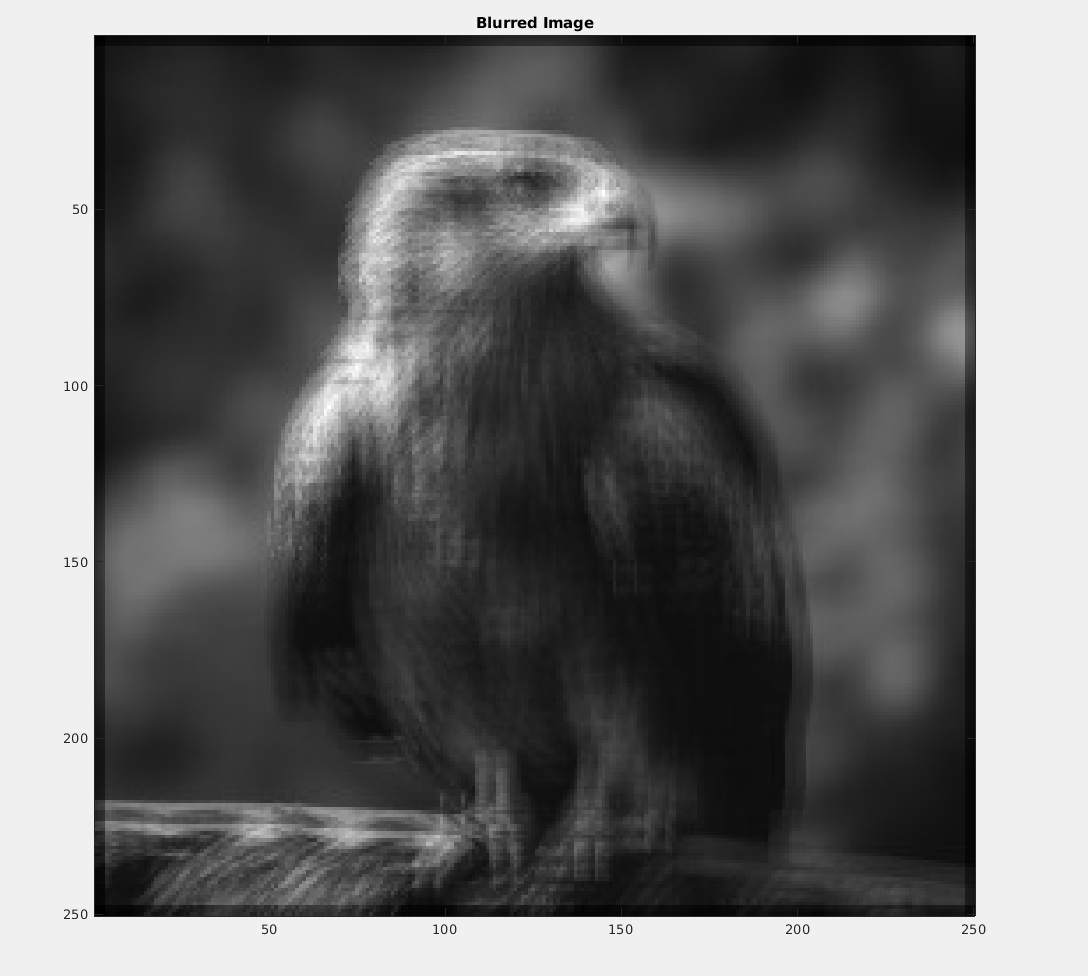
\includegraphics[width=0.4\linewidth]{./figures/ex4a2.png}
    \end{minipage}
  \caption{Original Blurred Image}
\end{figure}

 \begin{figure}[h!]
    \begin{minipage}[c]{1\linewidth}
        \centering
        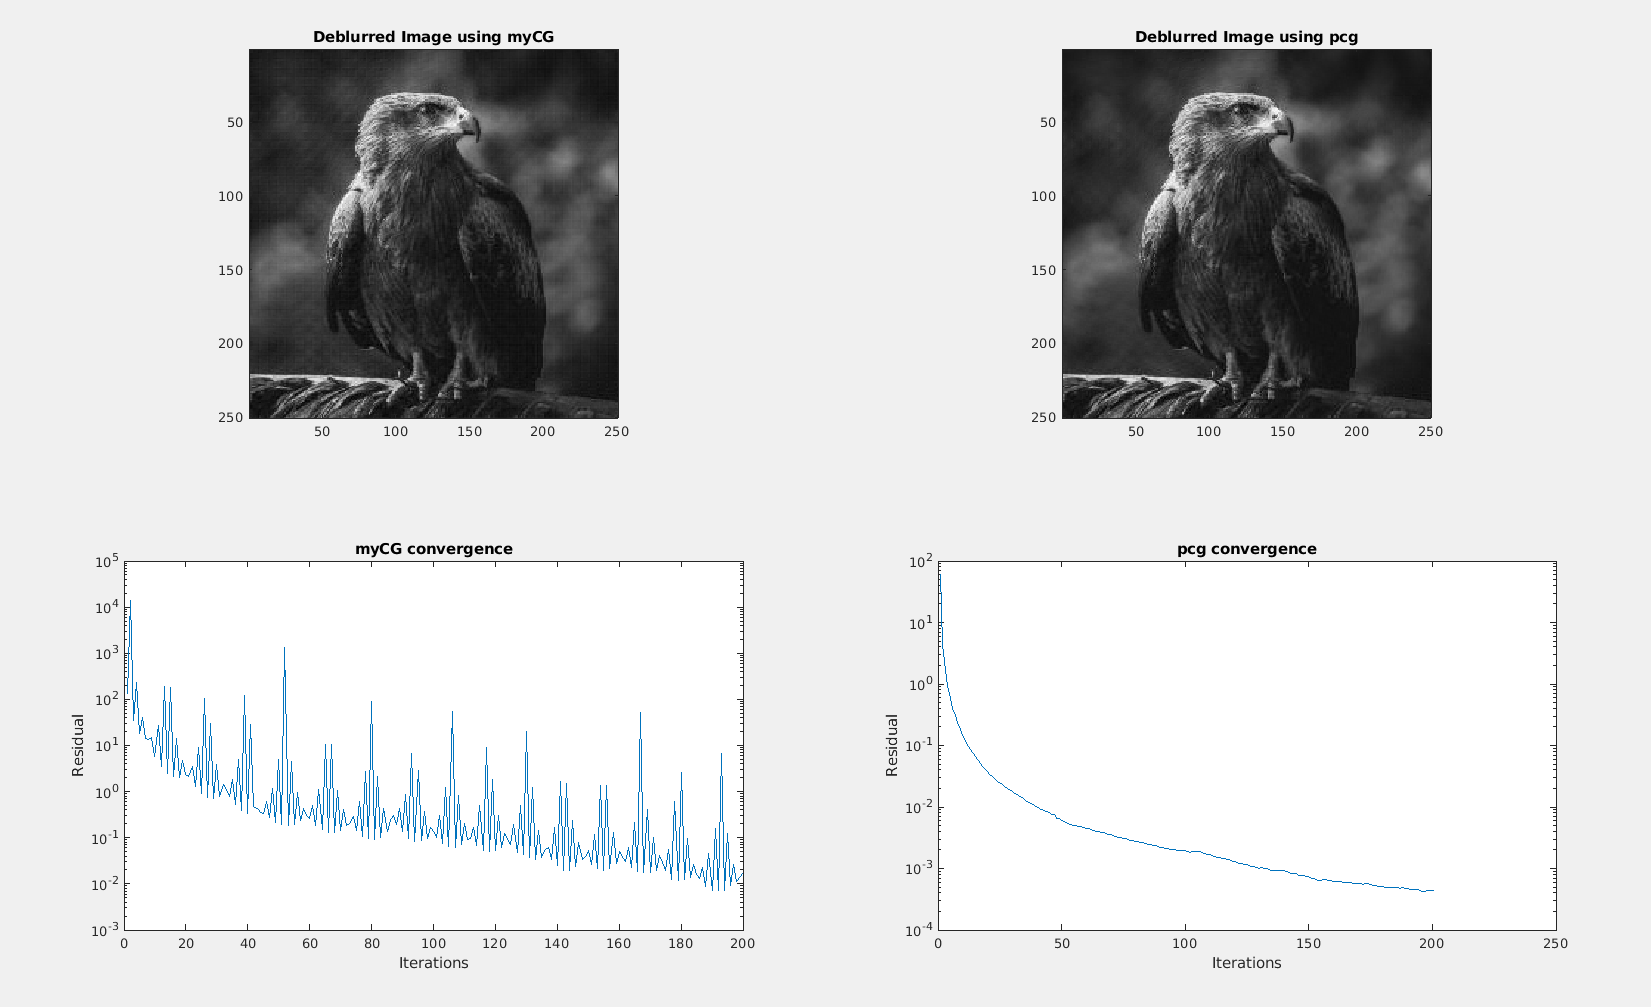
\includegraphics[width=0.9\linewidth]{./figures/ex4a.png}
    \end{minipage}
  \caption{Comparison of myCG function and pcg function (Top: image deblurring, Bottom: Convergence graph)}
\end{figure}

Image deblurred through ${pcg}$ shows more bluriness than the deblurred image obtained through ${myCG}$ method.To clarify, even though it is not absolutely clear, if viewed with focus, it is visible ${pcg}$ method does deblure the image. Which means deblurring through ${pcg}$ is not complete or less progressed in the given iteration limit. ${myCG}$'s convergence shows a similar trend to figure 1 computed before, monotonically decreasing. From the plotting of ${ResidualVSIteration}$ of ${pcg}$, it shows residual did show some decrease in residual overall, which indicates it does deblur the image but just in a slower pace of converging in comparison to ${myCG}$ implementation. From both the image and graph, it is clear ${myCG}$ implementation is more efficient than ${pcg}$ and ${pcg}$ has higher computational cost in an individual deblurring process.

\item When would pcg be worth the added computational cost? What about if you are deblurring lots of images with
the same blur operator? \\

PCG is particularly useful when dealing with ill-conditioned linear systems. It can mitigate the effects of ill-conditioning and improve the convergence rate compared to the standard Conjugate Gradient (CG) method (${myCG}$ method for example). Also, it is implemented in a way it would be easier to run it in a parallel computing architecture, which in modern world is faster than standard Conjugate Gradient method.

In case the same blur operator is used, PCG method is very efficient. The computational cost of setting up the preconditioner, (reutilized after calculating once) which is very costly, can be justified by the acceleration in convergence of images afterwards. The preconditioner is applied to the system matrix and helps improve its conditioning, leading to faster convergence of the PCG method.


\end{enumerate}




\end{document}
